% !TeX root = main.tex

\documentclass{article}
% Remove the footnote rule completely
\renewcommand{\footnoterule}{}
%%%%
\usepackage[english]{babel}
\usepackage{graphicx} % Required for inserting images
\graphicspath{{images/}}
\usepackage[export]{adjustbox}
\usepackage{wrapfig}
\usepackage[font=small,labelfont=bf]{caption}
%\usepackage[backend=biber, style=alphabetic, citestyle=authoryear]{biblatex}
\usepackage{tabularx}
\usepackage{multirow}
%\usepackage[hidelinks]{hyperref}

%\usepackage[numbers]{natbib}

\usepackage{subcaption}
\usepackage{multirow}
\usepackage{pdfpages}

\usepackage{siunitx}
\sisetup{locale = DE, quotient-mode = fraction, parse-numbers=false}
\usepackage{amssymb}
\usepackage{mathtools}
%%%%

\usepackage[english]{babel}
\usepackage{graphicx} % Required for inserting images
%\usepackage[a4paper]{geometry}
\usepackage{fancyhdr}
\usepackage{lastpage}
\usepackage{graphicx, wrapfig, subcaption, setspace, booktabs}
\usepackage[T1]{fontenc}
\usepackage{hyperref}
\usepackage{float} %Bildpositionierung
\setlength{\parindent}{0pt} %not sure
\usepackage[
  backend=biber,
  style=numeric,
  citestyle=numeric
]{biblatex}                     %Zitieren im IEEE Stil

\usepackage{csquotes}            %Zum Zietieren verwendetet package

\title{Bussystem und Sensorik - Smart Home Cube\ \vspace{2cm}}

\author{    
            \textbf{HAW Hamburg | Projectwork} René Bloeß }
\date{}


%%%%%%%%%%%%%%
%\lstset{style=mystyle}

%% Code Styling (End)

\usepackage{booktabs}

\usepackage{fancyhdr}
\usepackage{lastpage}
\usepackage[a4paper, top=4cm, bottom=4cm, left=3cm, right=3cm,
headheight=2cm, headsep=1cm, footnotesep=1cm]{geometry}
\pagestyle{fancy}

\usepackage{pgfplots}
\pgfplotsset{compat=1.16}

\usepackage{hyperref}
\hypersetup{
    colorlinks,
    citecolor=black,
    filecolor=black,
    linkcolor=black,
    urlcolor=black
}

\fancyhead{}

\usepackage{adjustbox}
\usepackage{makecell}
\usepackage{algorithm}
\usepackage{algpseudocode}
\usepackage{tikz}

\lhead{\raisebox{0.75\height}{BU}}
\chead{\raisebox{0.75\height}{Smart-Home-Cube}}
\rhead{\raisebox{0.75\height}{Oktober 2025}} 

\fancyfoot{}
\lfoot{R. Bloeß}
\cfoot{Seite \thepage\ von \pageref{LastPage}}
\rfoot{\raisebox{-0.3\height}{
\includegraphics[height=1cm]{images/haw-logo.jpg}}}
\renewcommand{\footrulewidth}{0.5pt}

\addbibresource{chapters/literature.bib} % Deine .bib Datei
%%%%%%%%%%%%
\begin{document}
\maketitle

\newpage
\tableofcontents
\section{Idee und Konzept}
Ich hatte schon immer den Traum, eines Tages mein eigenes Elektronikprodukt zu entwickeln, es zum Leben zu erwecken und bis zu einem kleinen kommerziellen Maßstab zu verkaufen.
Natürlich fand ich dabei besonderes Interesse im Bereich Smart Home sowie bei elektronischen Spielzeugen und Gadgets.
Hier kam mir ursprünglich die Idee eines würfelförmigen Spielzeugs, das aus einem Mikrocontroller und einem modernen \textcolor{blue}{OLED}-Display besteht, auf dem eine Art Tamagotchi dargestellt wird.
Dies ist natürlich ein Konzept, das bereits weit verbreitet ist und ohne erheblichen Marketingaufwand sowie besondere Alleinstellungsmerkmale kaum verkäuflich wäre.
\\\\
Trotz dieses Wissens wollte ich dennoch etwas Ähnliches umsetzen. So entstand die Idee des Smart-Home-Cubes \textbf{(SHC)}.
Kurz gesagt teilt er das gleiche äußere Erscheinungsbild, das ich mir für meine ursprüngliche Spielzeugidee vorgestellt hatte,
ist jedoch einfach ein Würfel, der mit allen erdenklichen Sensoren ausgestattet ist.
Alle diese Informationen sollen in Echtzeit übersichtlich auf dem \textcolor{blue}{OLED}-Frontdisplay dargestellt werden.
Zudem besteht die Möglichkeit zur Tasteninteraktion, um beispielsweise auf Abruf Mittelwerte von Temperatur oder Luftfeuchtigkeit anzuzeigen.
\\\\
Alle verschiedenen Sensoren sollen in Echtzeit ausgelesen und kontinuierlich ausgewertet werden.
Im Konzept sind sie alle an dieselbe \textcolor{blue}{I2C}-Busleitung angeschlossen.
Eine Übersicht aller Ziele ist unten dargestellt.
\subsection{Konzept Übersicht}
\begin{table}[h!]
\centering
\renewcommand{\arraystretch}{1.3}
\begin{tabularx}{\textwidth}{|l|X|X|}
\hline
\textbf{Kategorie} & \textbf{Ziel / Feature} & \textbf{Beschreibung} \\
\hline
\multirow{7}{*}{\textbf{Haupt Ziele}} 
    & Custom ESP32-S3 PCB Design      & Kern des Projektes \\
    & USB-C Support                   & Power + Data via USB-C \\
    & Feuchtigkeitssensor Sensor                 & Umgebungserfassung \\
    & Temperatur Sensor              & \\
    & Druck Sensor                 & \\
    & Strom Monitoring              & Stromverbrauch messung \\
    & Real-time OLED Display (1x)     & Echtzeitdarstellung der Messwerte \\
\hline
\multirow{7}{*}{\textbf{Optionale Ziele}}
    & 3D Case Design                  & 3D Gedruckt \\
    & 3× OLED Screens                 & Mehr Visuelles Feedback \\
    & Licht  Sensor                    & \\
    & UV Sensor                       & \\
    & CO\textsubscript{2} Sensor      & \\
    & Interaktive Sensor Interpretation & Dynamische, Steuerung(Knöpfe) \\
    & Daten speicherung \& Durchschnitt  & Historical statistics \\
\hline
\end{tabularx}
\caption{Übersicht der Haupt- und Nebenziele}
\end{table}
\newpage
\subsection{Visuelle Darstellung der Idee}
\begin{figure}[h]
    \centering
    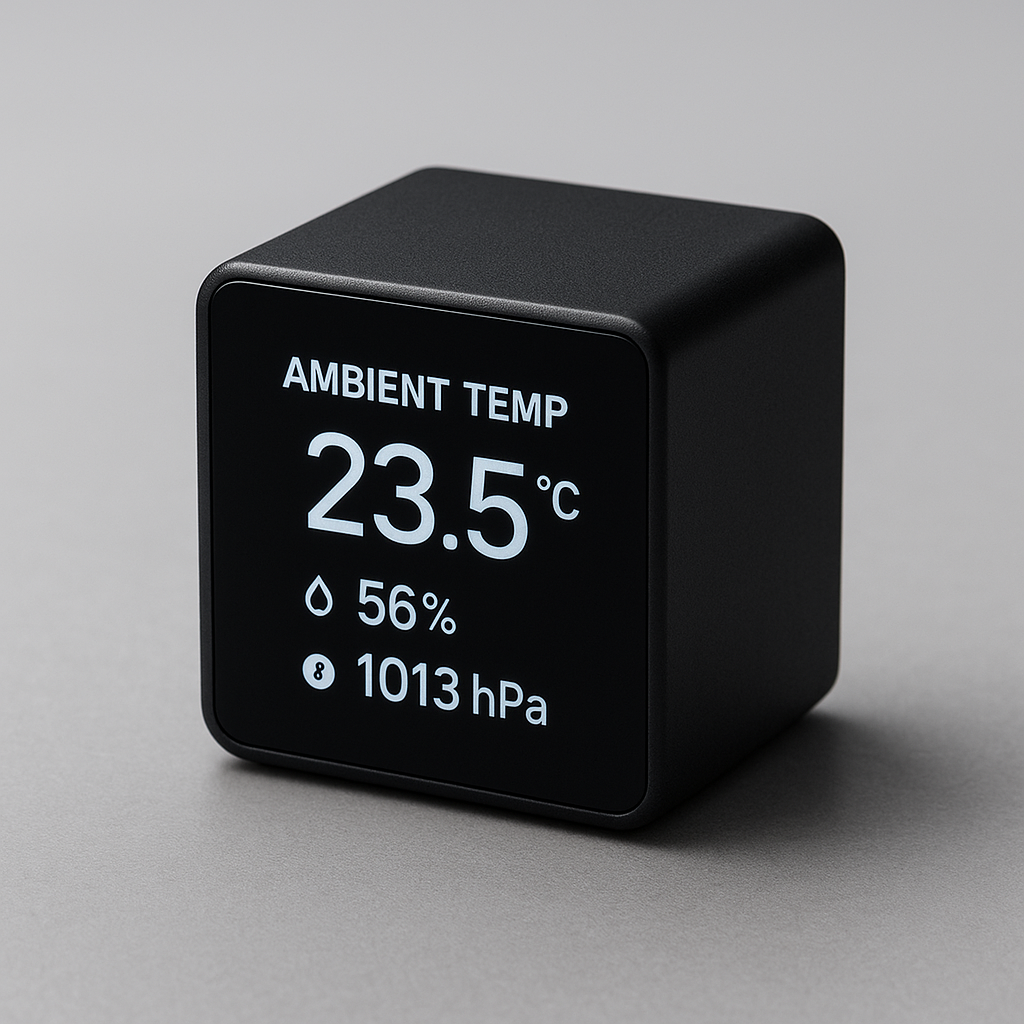
\includegraphics[width=1\linewidth]{images/cube.png}
    \caption{Concept Art\protect\footnotemark}
    \label{fig:v24}
\end{figure}
\footnotetext{Dieses bild wurde mithilfe von  OpenAI-GPT-5 generiert}
\newpage
\begin{figure}[h]
    \centering
    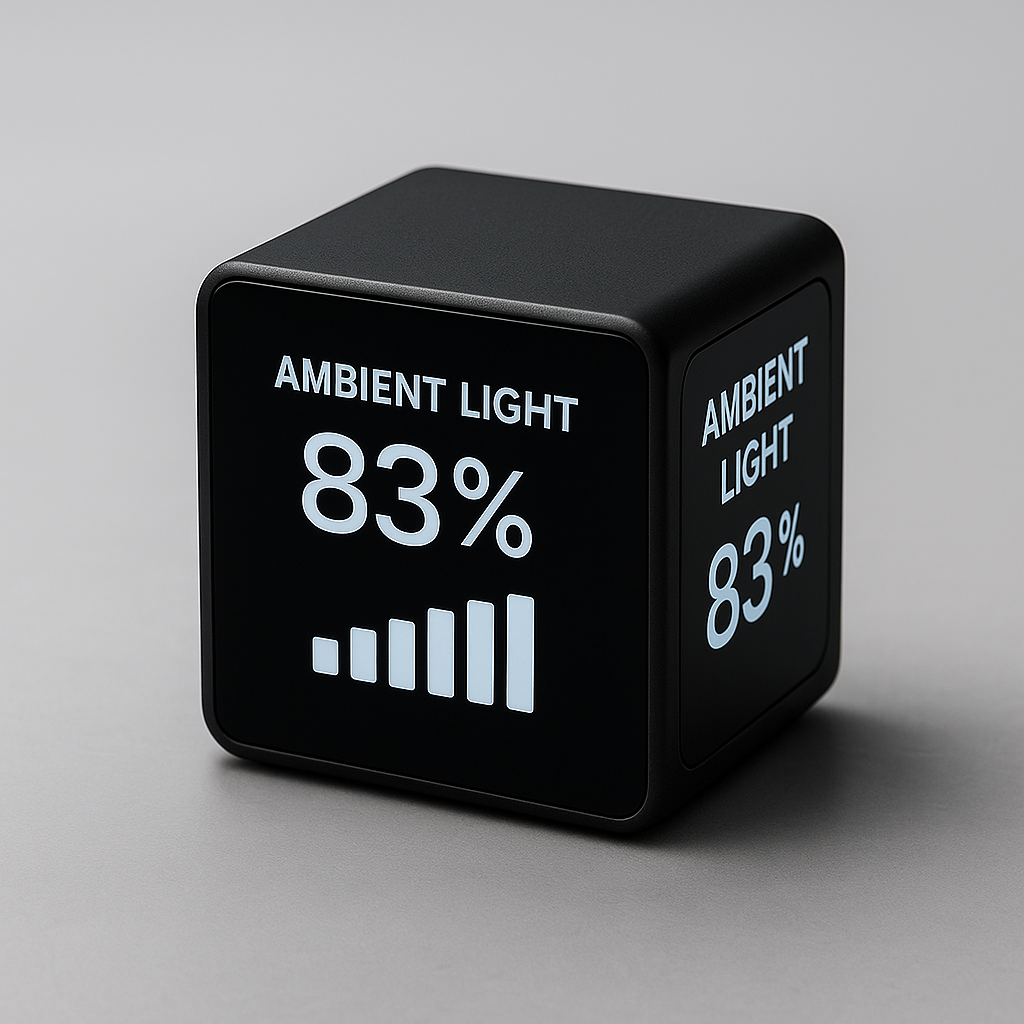
\includegraphics[width=1\linewidth]{images/cube2.png}
    \caption{Concept Art\protect\footnotemark}
    \label{fig:v24}
\end{figure}
\footnotetext{Dieses bild wurde mithilfe von  OpenAI-GPT-5 generiert}
\newpage
\begin{figure}[h]
    \centering
    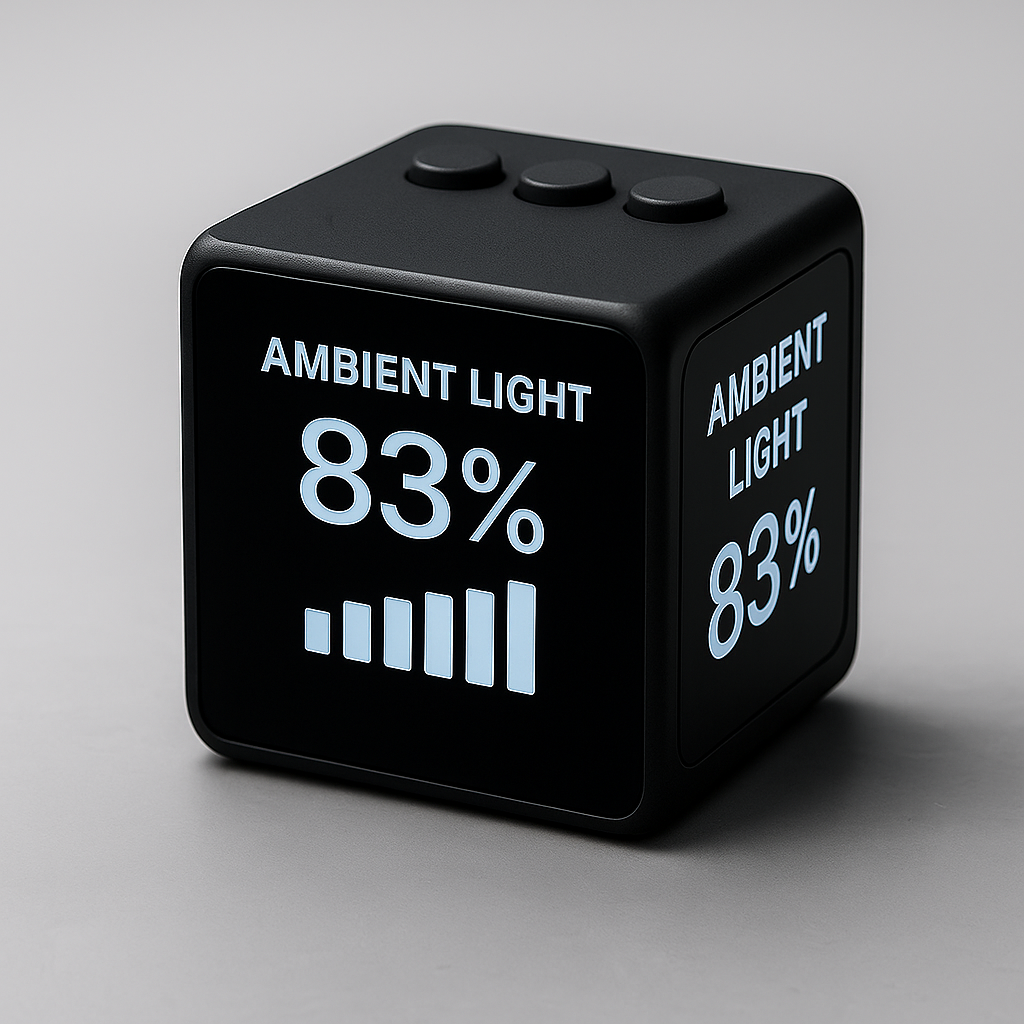
\includegraphics[width=1\linewidth]{images/cube3.png}
    \caption{Concept Art\protect\footnotemark}
    \label{fig:v24}
\end{figure}
\footnotetext{Dieses bild wurde mithilfe von  OpenAI-GPT-5 generiert}
\newpage
\begin{figure}[h]
    \centering
    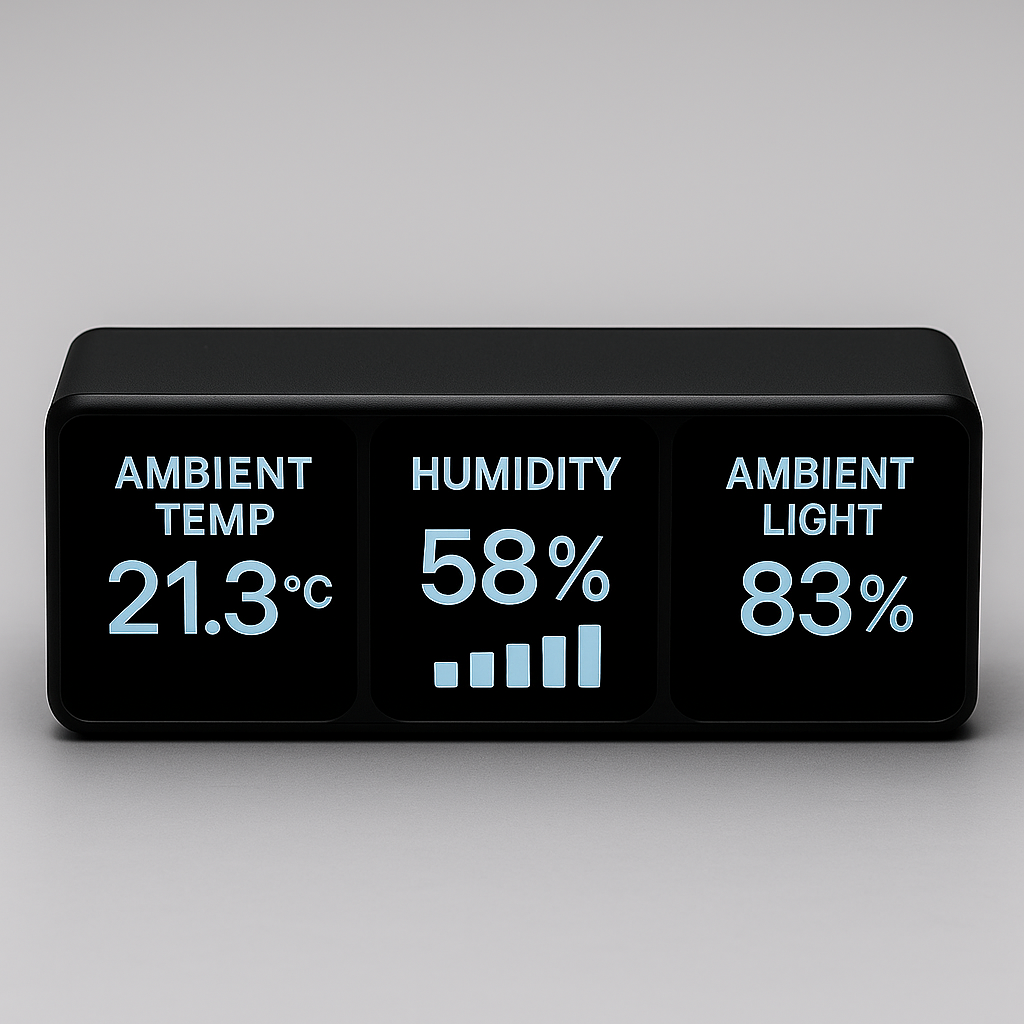
\includegraphics[width=1\linewidth]{images/cube4.png}
    \caption{Concept Art\protect\footnotemark}
    \label{fig:v24}
\end{figure}
\footnotetext{Dieses bild wurde mithilfe von  OpenAI-GPT-5 generiert}









\section{Schematic und PCB}
\subsection{ESP32-S3}
Wie bereits zuvor besprochen, soll eine eigenes PCB entwickelt werden, um alle Geräte darauf unterzubringen.
Im Zentrum der Platine wird sich das \textbf{ESP32-S-WROOM-1} Modul befinden. Es läuft mit bis zu 240 MHz und ist mit einem 2,4 GHz-Transceiver ausgestattet,
der potenziell \textcolor{blue}{Bluetooth}- oder \textcolor{blue}{WIFI}-Unterstützung bietet.
Mit 36 verfügbaren GPIO-Pins stehen uns zahlreiche Möglichkeiten für zusätzliche Funktionen offen.

\begin{figure}[ht]
    \centering
    \begin{subfigure}{0.45\textwidth}
        \centering
        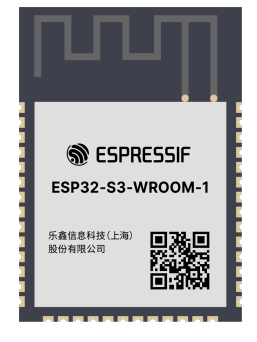
\includegraphics[width=\textwidth]{images/ESP32-S3.png}
        \caption{Top view}
        \label{fig:image1}
    \end{subfigure}
    \hfill
    \begin{subfigure}{0.50\textwidth}
        \centering
        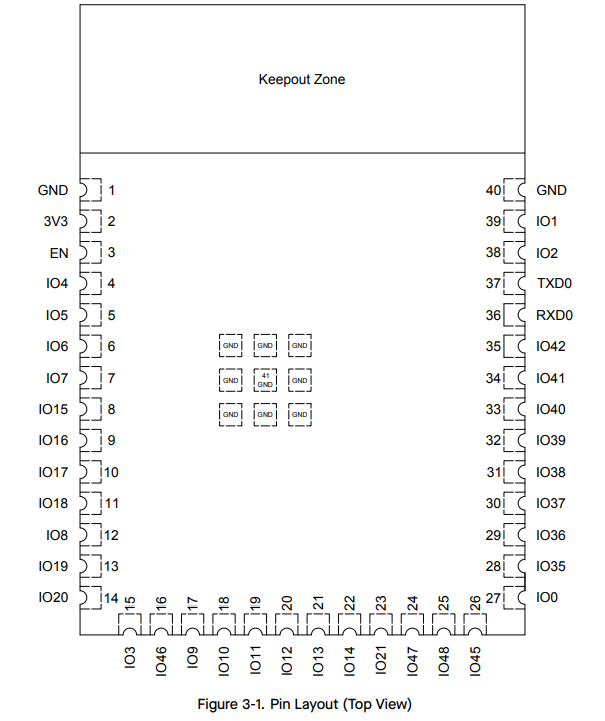
\includegraphics[width=\textwidth]{images/ESP32-S3-schem.png}
        \caption{Schematic}
        \label{fig:image2}
    \end{subfigure}
    \caption{ESP32-S3-WROOM-1}
    \label{fig:both_images}
\end{figure}
\newpage
\subsection{Stromversorgung und Kommunikation}


Zu unserem vorteil, besistz der \textbf{ESP32-S-WROOM-1} native \textbf{USB 2.0} Unterstützung. Diese tatsache ermöglicht
es uns per USB mit dem Modul zu kommunizieren und gleichzeitig die Platine zu versorgen. Um nun dennoch die Vroteile der kompatibilität
von USB-C anstatt USB 2.0 nutzen zu könnnen, sind einige dinge bei der Auslegung zu beachten. Hierbei können wir  die 
\textcolor{red}{CCx (A5,B5)} termination Pins des Steckers nutzen um unseren Stromverbrauch, gemäß der USB-C Spezifikation 
den Host Device bekannt geben ohne einen Powercontroll-IC zu benötigen mit lediglich  10k\si{\ohm} pulldowns zu GND.
Des weiteren nutzen wir weiterhin für die kommunikation die \textbf{USB 2.0} Pins \textcolor{red}{D+, D- (A6,B6,A7,B7)}.

\begin{figure}[h]
    \centering
    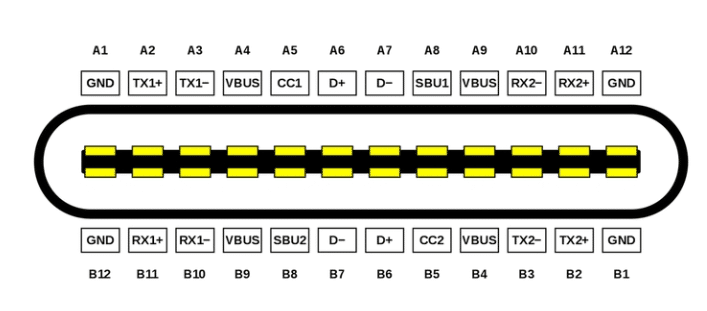
\includegraphics[width=1\linewidth]{images/usbcpinout.png}
    \caption{USB-C Pinout}
    \label{fig:v24}
\end{figure}

\begin{figure}[h]
    \centering
    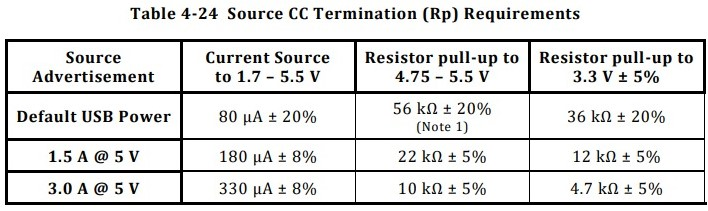
\includegraphics[width=1\linewidth]{images/usbc.png}
    \caption{USB-C Power request}
    \label{fig:v24}
\end{figure}
\newpage
Durch die vorherigen besprochenen methoden kommt folgendes Schematic zustande. 
\begin{figure}[h]
    \centering
    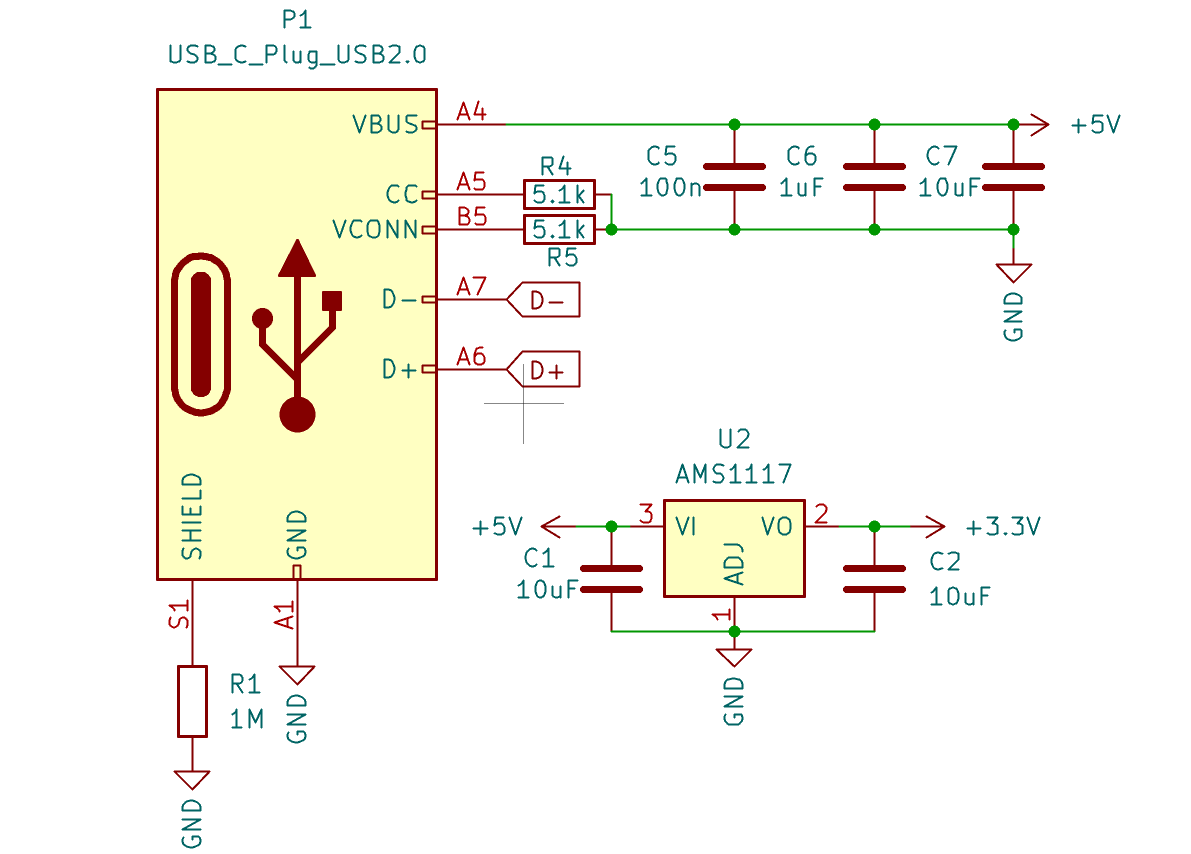
\includegraphics[width=1\linewidth]{images/usbcsch.png}
    \caption{USB-C Schematic}
    \label{fig:v24}
\end{figure}
\\



Zusätzlich müssen wir uns außer die native 5V Spannung von USB-C ebenfalls eine 3.3V versorgungsspannung erzeugen, die den
\textbf{ESP32-S-WROOM-1}, sowie die Sensoren mit Spannung versorgt. Hierfür nutze ich den \textbf{AMS1117} Low-Dopout-Regulator(LDO).
Dieser wandelt die übrige Spannung die in ihnen eingespeißt wird in wärme um, was es ihm erlaubt eine 3.3V Ausgangsspannung zu erzeugen
mit einem Maximal Strom von bis zu 1A, was mehr als genug ist für unseren ESP32 und die restlichen komponennten.

\newpage
\subsection{I$^{2}$C  Busslinie und Sensoren}
Um nun die gewollte funktion der Umgebungserfassung zu gewährleisten sind natürlich Sensoren erforderlich. Die kriterien
nach denen ich diese ausgewählt habe sind wie folgt:\\

$\cdot$ 3.3V Kompatibel\\
$\cdot$ I${^2}$C Kompatibel\\
$\cdot$ günstig und verfügbar als Modul\\\\

Dabei habe ich mich für folgende Komponennten entschieden.

\begin{table}[h]
\centering
\caption{Übersicht der Sensoren und ihrer Funktionen}
\label{tab:sensoren}
\begin{tabular}{>{\raggedright\arraybackslash}p{3cm}>{\raggedright\arraybackslash}p{8cm}}
\toprule
\textbf{Sensor} & \textbf{Funktion} \\
\midrule
BMP390 & Hochpräziser digitaler Luftdrucksensor mit sehr niedrigem Rauschen. Misst den absoluten Luftdruck. Wird häufig für Höhenmessung, Wetterstationen und IoT-Anwendungen verwendet. \\
\addlinespace
INA219AxD & Bidirektionaler Gleichstrom-Messverstärker mit I\textsuperscript{2}C-Schnittstelle. Misst Spannung, Strom und Leistung über einen Shunt-Widerstand. Ideal für Energieverwaltungssysteme. \\
\addlinespace
LM75B & Digitaler Temperatursensor und Thermostat mit I\textsuperscript{2}C-Schnittstelle. Misst Temperaturen von -55°C bis +125°C mit einer Genauigkeit von ±2°C. Einfache Plug-and-Play-Lösung. \\
\addlinespace
SHTC3 & Digitaler Feuchtigkeitssensor mit I\textsuperscript{2}C-Schnittstelle. Bietet hohe Genauigkeit bei niedrigem Stromverbrauch. Ideal für HVAC-Systeme und Wetterüberwachung. \\
\bottomrule
\end{tabular}
\end{table}

\newpage

\begin{figure}[h]
    \centering
    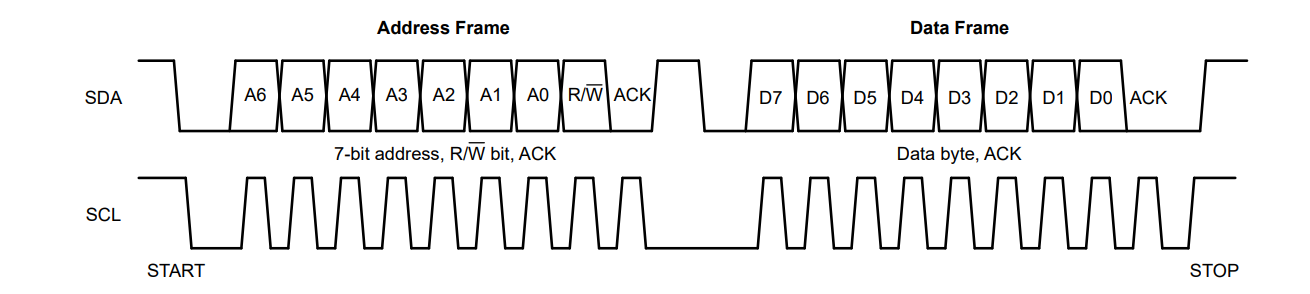
\includegraphics[width=1\linewidth]{images/i2cwork.png}
    \caption{I2C Adress and Data Frames \cite{I2C}}
    \label{fig:v24}
\end{figure}







\printbibliography

%\counterwithout{section}{chapter}

\newpage

\end{document}